\section{Architettura}
\subsection{Pattern architetturale: MVC}
\begin{figure}[H]
    \centering
    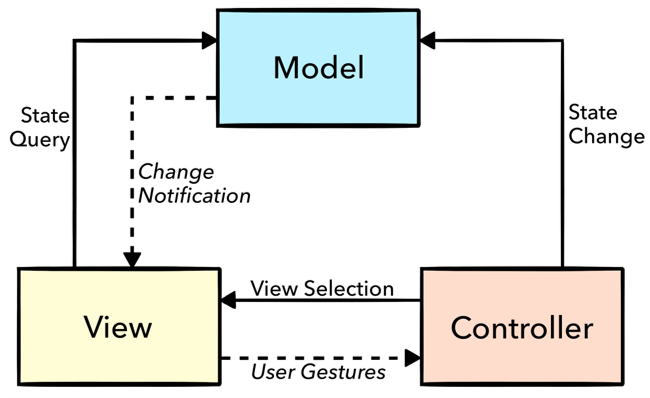
\includegraphics[scale = 1]{components/img/mvc-generico.png}
    \caption{Diagramma pattern MVC}
    \label{fig:diagramma MVC generico}
\end{figure}
L'architettura del capitolato C7 aderisce al pattern architetturale \textit{Model-View-Controller (MVC).} L'aderenza al pattern era un requisito obbligatorio imposto dall'azienda ma sono stati riscontrati diversi punti positivi nella sua implementazione:

\begin{itemize}
	\item Rapidità nello sviluppo software dato dalla possibilità di lavoro parallelo su modello, vista e controller;
	\item Indipendenza dei vari componenti;
	\item Maggior facilità nella testabilità, mantenibilità e scalabilità.

\end{itemize}
\subsection{Diagramma dei pacchetti}
\begin{figure}[H]
    \centering
    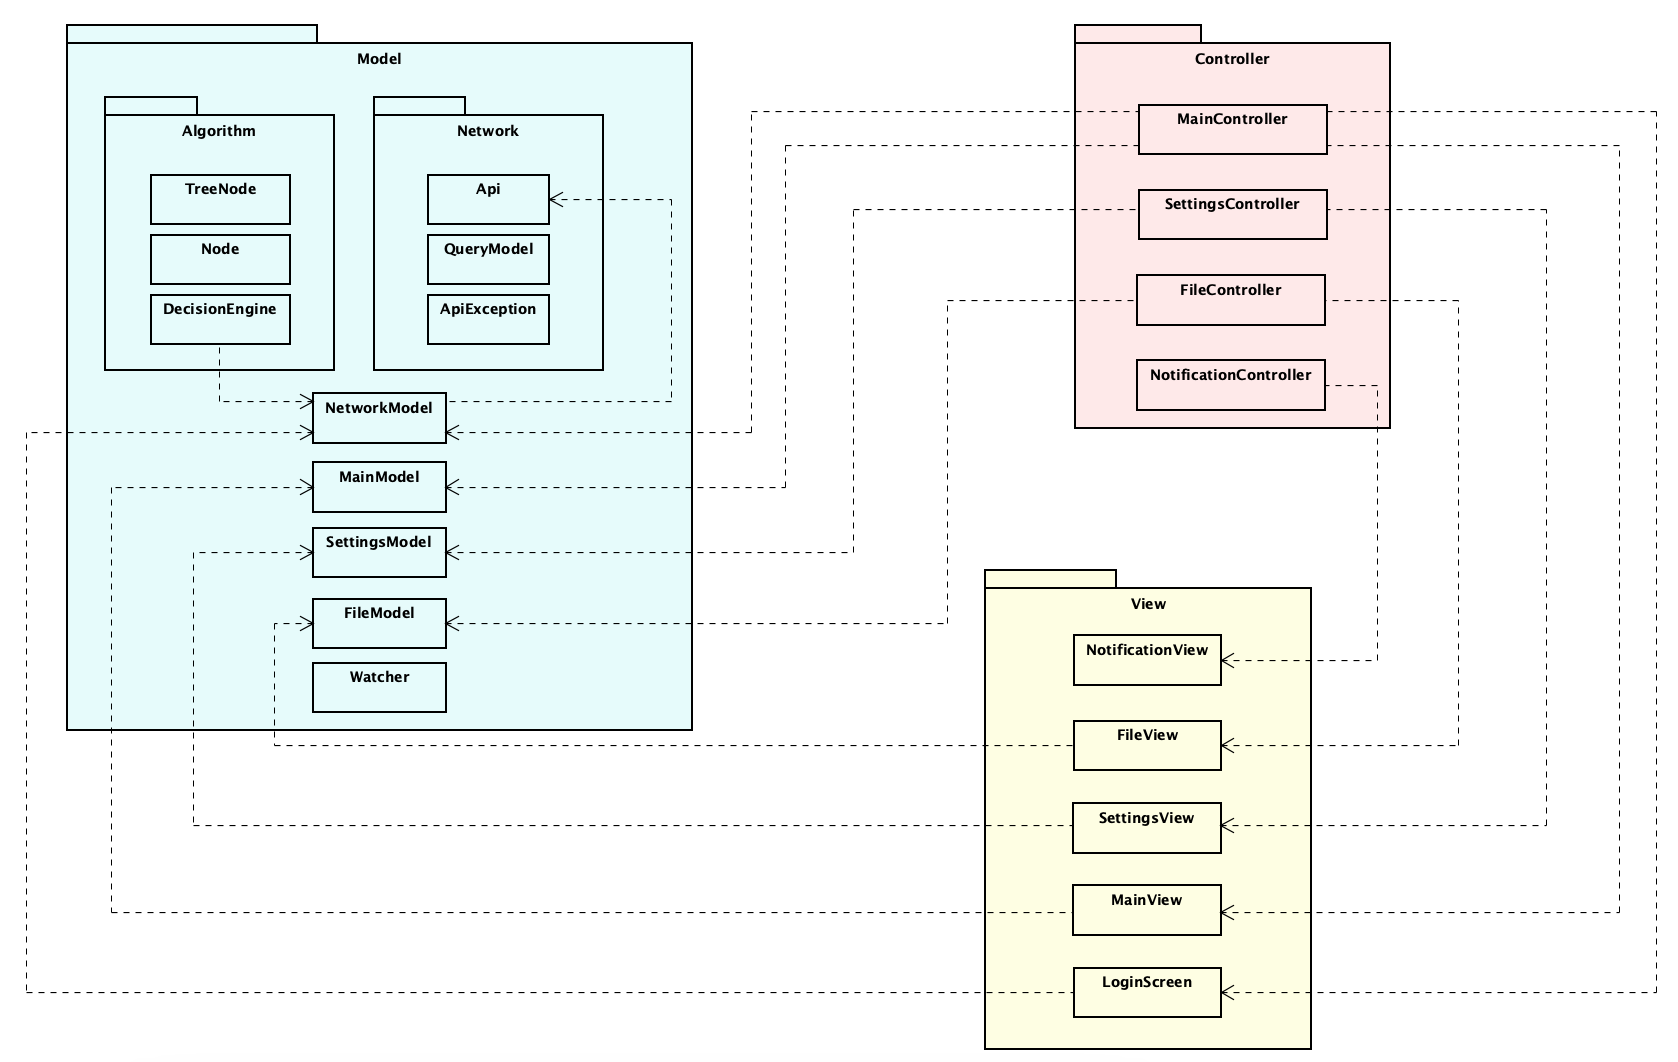
\includegraphics[scale = 1]{components/img/diagramma-package.png}
    \caption{Diagramma pacchetti}
    \label{fig:diagramma pacchetti}
\end{figure}
\subsection{Diagramma delle classi - model}

\begin{figure}[H]
    \centering
    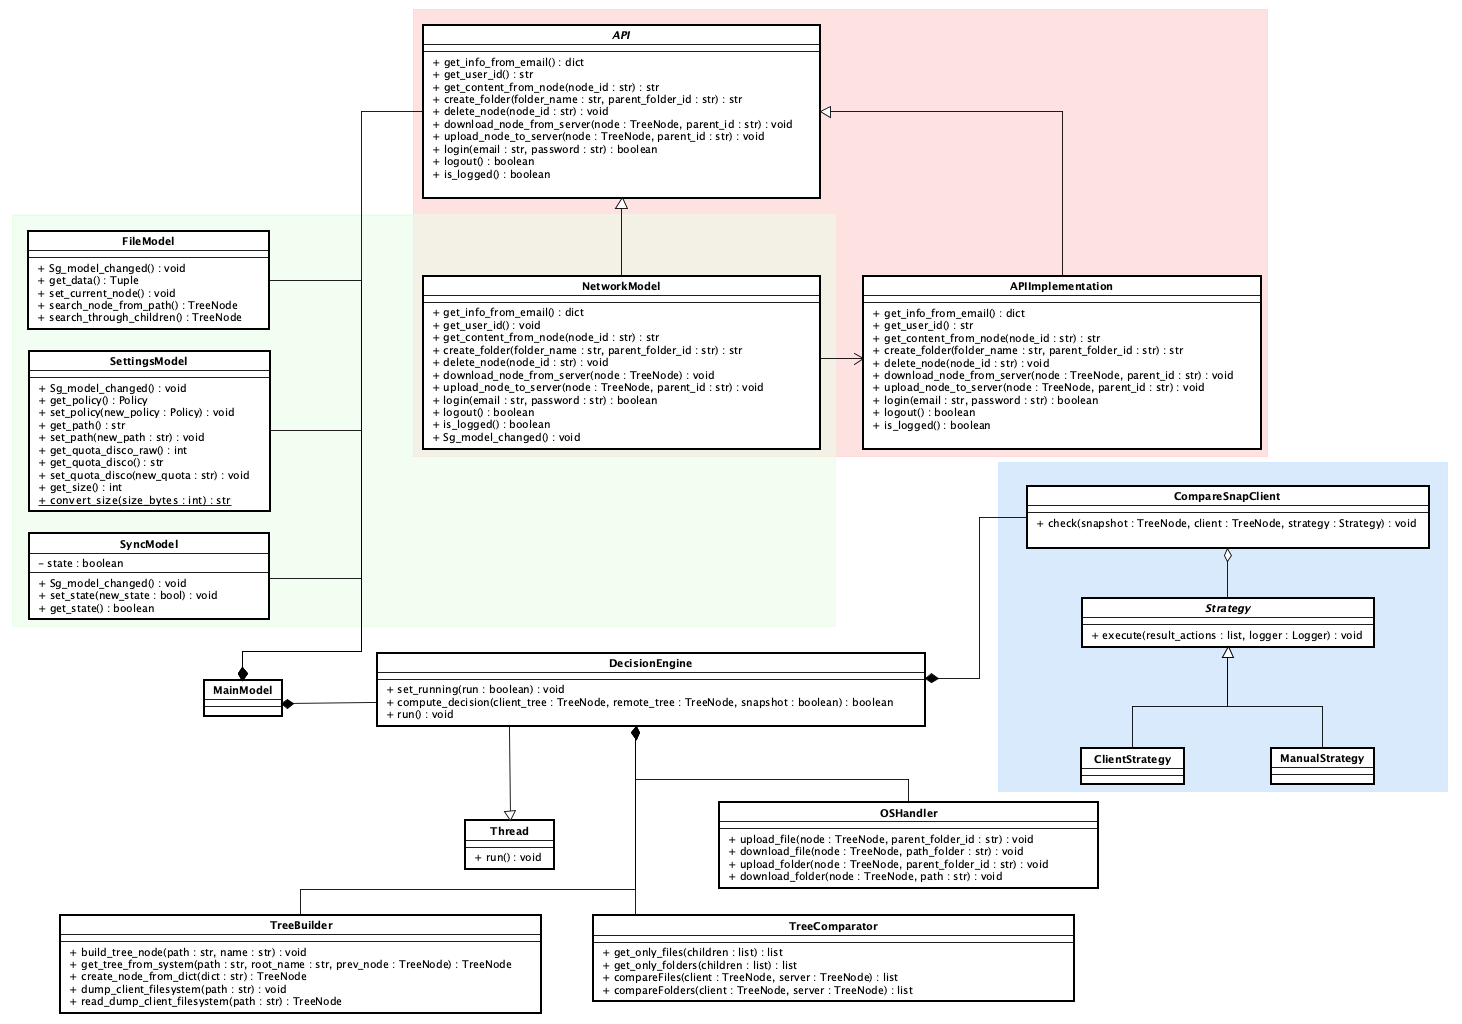
\includegraphics[scale = 0.8]{components/img/diagramma-classi-model.png}
    \caption{Diagramma delle classi nel model}
    \label{fig:Diagramma delle classi nel model}
\end{figure}

\subsection{Design pattern creazionali: Singleton}

Tutte queste quattro classi rispettano il pattern singleton, andando quindi ad avere una sola loro istanza all'interno del programma. Questo in Python è stato realizzato tramite del codice specifico che va a definire un comportamento nel quale le varie classi possono essere instanziate solamente tramite la funzione get\_instance ed il costruttore non può essere chiamato al di fuori di questa funzione. La funzione get\_instance controlla se è la classe è già stata istanziata, se non è stato istanziata crea una nuova istanza e nelle chiamate successive si limita a restituire nuovamente la stessa.\newline{}
Il pattern singleton può provocare problemi se mal implementato, attualmente l'implementazione è corretta dato che l'istanza dei vari modelli è passata ai costruttori di tutti gli utilizzatori. Questo permette la realizzazione degli unit test che altrimenti sarebbero impossibili da implementare. 
\begin{figure}[H]
    \centering
    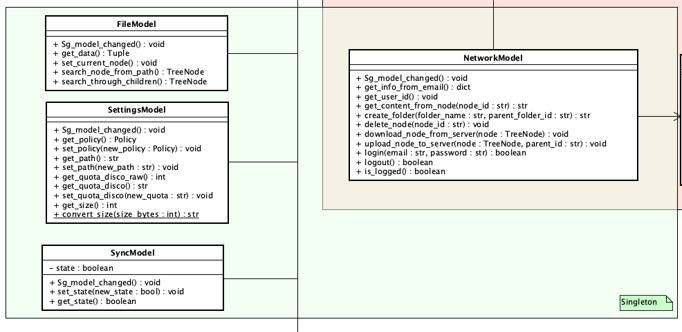
\includegraphics[scale = 0.8]{components/img/singleton-model.png}
    \caption{Diagramma del pattern singleton}
    \label{fig:Diagramma del pattern singleton}
\end{figure}
\subsection{Design pattern strutturali: Virtual Proxy}
Il pattern Proxy viene utilizzato per evitare chiamate di rete non necessarie, permettendo la lazy initialization.\newline{}
Questo pattern in python è stato realizzato tramite il modulo ABC (Abstract Base Classes) che ci permette di andare a definire delle classi astratte. Si è quindi realizzata la classe astratta API che viene ereditata da NetworkModel e da APIImplementation,andando quindi a definire dei metodi base che entrambe le classi condividono. Quando verrà effettuata una chiamata di rete si andrà quindi a passare per il network model che dopo controlli aggiuntivi potrà decidere se passare la chiamata ad ApiImplementation. Network model è quindi il nostro proxy e ApiImplementation il nostro realsubject.
\begin{figure}[H]
    \centering
    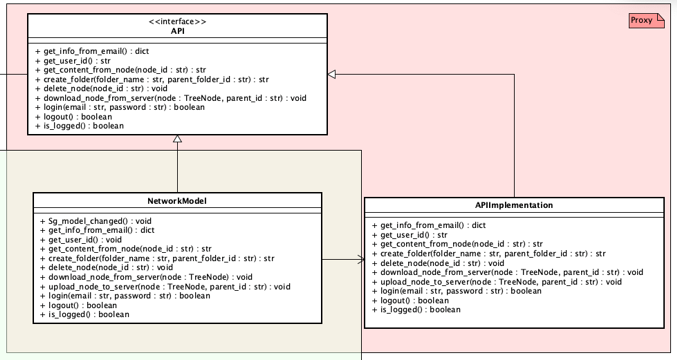
\includegraphics[scale = 0.8]{components/img/proxy-model.png}
    \caption{Pattern proxy nel dettaglio}
    \label{fig:Pattern proxy nel dettaglio}
\end{figure}
\subsection{Design pattern comportamentali:}
\subsubsection{Observer:}
\begin{figure}[H]
    \centering
    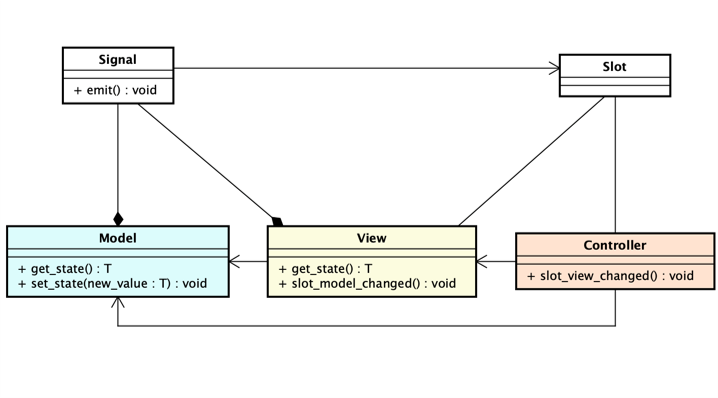
\includegraphics[scale = 1]{components/img/observer-implementazione.png}
    \caption{Pattern observer con segnali e slot}
    \label{fig:Pattern observer con segnali e slot}
\end{figure}

*CORREGGERE LINEE DA SLOT A VIEW/C

*PICCOLA SPIEGAZIONE SULL'USO DEI SEGNALI *

\subsubsection{Strategy:}
L'utilizzo di questo pattern è stata una scelta naturale poichè esso va a descrivere pienamente la realtà del \textit{capitolato C7}.\newline{}
Attualmente si hanno due diverse politiche per la sincronizzazione che posso essere scelte in runtime e che variano il comportamento dell'algoritmo. Si ha una classe Context che fà da interfaccia comune e chiama al suo interno il metodo execute della strategy attualmente scelta. Essendo Strategy una classe astratta essa fornisce il metodo execute che deve essere implementato da tutte le classi figlie. Questo permette all' istanza di Context di poter chiamare il metodo execute di un qualsiasi oggetto strategy di cui non conosce l'implementazione. Possono quindi essere aggiunte con sviluppi futuri nuove politiche con le corrispondenti classi che ereditano da Strategy senza dover cambiare la logica dell'applicazione.

\begin{figure}[H]
    \centering
    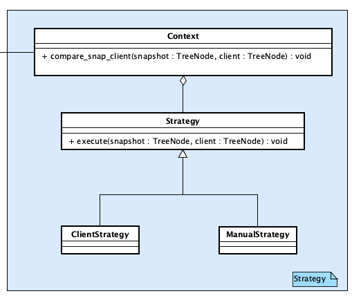
\includegraphics[scale = 0.8]{components/img/strategy-model.png}
    \caption{Pattern proxy nel dettaglio}
    \label{fig:Pattern proxy nel dettaglio}
\end{figure}
